\section{Zielsetzung}
Mittels eines Lasers kann kohärentes und monochromatisches Licht erzeugt werden. In diesem Versuch soll die Funktionsweise eines Diodenlasers untersucht sowie mithilfe eines solchen Lasers das Absorptionsspektrum von Rubidium vermessen werden.
\section{Theorie}
\label{sec:Theorie}
\subsection{Halbleiter}
In Festkörpern sind aufgrund des Pauli-Verbots die eigentlich diskreten Energieniveaus der Atome in kontinuirliche Bänder aufgespalten. Wenn das oberste energetische Band nicht voll besetzt ist können sich Elektronen frei bewegen und es handelt sich um einen Leiter. Wenn das letzte besetzte Band voll ist wird das höchstenergetische voll besetzte Band als Valenzband und das darüberliegende leere Band als Leitungsband bezeichnet. 
\begin{figure}[h]
\centering
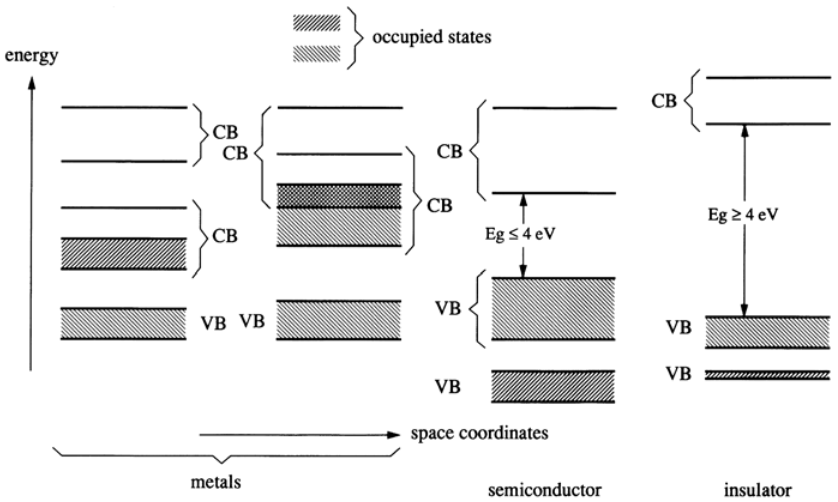
\includegraphics[width=0.8\textwidth]{Bandschema}
\caption{Bandschema für ein Metal (links), Isolator (mitte) und Halbleiter (rechts). Isolator und Halbleiter unterscheiden sich durch die Größe der jeweiligen Bandlücke.\cite{Semiconductor_Optics}}
\label{fig:Bandschema}
\end{figure}
Je nach Größe der sogenannten Bandlücke zwischen Valenz- und Leitungsband handelt es sich bei einer großen Bandlücke um einen Isolator und bei einer kleineren Bandlücke um einen Halbleiter. In letzterem Falle können Elektronen durch thermische Anregung die Bandlücke überwinden wodurch das Material leitend wird. Die Bandstruktur in den verschiedenen Fällen ist in Abbildung $\ref{fig:Bandschema}$ illustriert.

Durch eine Dotierung des Halbleiters kann die Leitfähigkeit weiter beeinflusst werden. Bei einer p-Dotierung werden dem Material Elektronen-Akzeptoren hinzugefügt, welche Elektronen aus dem Valenzband aufnehmen und somit für zusätzliche Löcher im Valenzband sorgen. Bei einer n-Dotierung werden dem Material Elektronen-Donatoren hinzugefügt, die zusätzliche Elektronen in das Leitungsband abgeben. Wenn ein p und ein n-dotierter Halbleiter aneinander liegen entsteht and der Grenzfläche ein sogenannter p-n-Übergang. An diesem Übergang entsteht eine Raumladungszone. Wenn an den Übergang eine externe Spannung angelegt wird kann diese Raumladungszone verstärkt werden und wie ein Isolator wirken oder überwunden werden und einen Ladungstransport ermöglichen.
\subsection{Besetzungsinversion und stimulierte Emission}
Bei dem Übergang eines Elektrons zwischen zwei Energieniveaus wird ein Photon emittiert oder absorbiert dessen Wellenlänge der Energiedifferenz des Übergangs gemäß $E=hf$ mit dem Planckschen Wirkungsquantum $h$ entspricht.
Dabei kann grundsätzlich zwischen drei unterschiedlichen Prozessen unterschieden werden. Bei der Absorption wird ein Photon vernichtet und regt dabei einen Übergang in ein höheres Energieniveau an. Bei der spontanen Emission geht ein Elektron in einen niedrigeren Energiezustand über und emmitiert dabei ein Photon.
Ein Photon kann auch an einem Atom einen Übergang und somit die Emission eines weiteren Photons mit identischer Wellenlänge, Phase und Polarisation zum anregenden Photon erzeugen. Durch diesen Prozess der stimulierten Emission wird die Verstärkung in einem Laser gewährleistet indem der Laser durch einen Resonator immer wieder die Emission neuer Photonen stimuliert und somit verstärkt wird. Damit die stimulierte Emission der dominierende Prozess ist und somit ein Verstärkungsprozess stattfindet muss das höherenergetische Energieniveau stärker besetzt sein als das niedrigere Niveau, eine sogenannte Besetzungsinversion, da ansonsten durch Absorption keine Verstärkung stattfinden kann. Um eine Besetzungsinversion gewährleisten zu können muss jedoch ein System mit mindestens drei Zuständen vorliegen, da sich die Zustände ansonsten durch spontane Emission entladen. Bei modernen Lasern werden in aller Regel Systeme mit vier Zuständen verwendet. 
\subsection{Funktionsweise eines Diodenlasers}
Ein beispiel für ein solches vier-Zustandssystem ist auch der Diodenlaser.
\begin{figure}[h]
\centering
\includegraphics[width=0.5\textwidth]{p-n-Übergang}
\caption{Photonemission am p-n-Übergang.\cite{Atoms}}
\label{fig:p-n-Übergang}
\end{figure}
Durch Anlegen einer äußeren Spannung am p-n-Übergang fließt ein Strom, wodurch Elektronen aus dem Leitungsband des n-dotierten Teils in den p-dotierten Teil verschoben werden. Umgekehrt werden auch die Löcher aus dem Valenzband des p-dotierten Halbleiters in Richtung des n-dotierten Teils verschoben Diese Elektronen können dann mit den Löchern im Valenzband rekombinieren, weshalb die Energie der induzierten Emission ungefähr der Bandlücke des Materials entspricht. Da es sich allerdings um Bänder und nicht um diskrete Energieniveaus handelt ist die Frequenz noch recht breit um das Maximum verteilt. Dieser Prozess ist in Abbildung $\ref{fig:p-n-Übergang}$ dargestellt. Da die aktive Schicht des p-n-Übergangs von dotierten Schichten mit höherer Bandlücke umgeben ist bestehen die vier Zustände des Systems hier also aus dem Leitungsband der Halbleiterschicht mit höherer Bandlücke und dem Leitungsband des aktiven p-n-Übergangs mit geringerer Bandlücke sowie wiederum dem jeweiligen Valenzband der aktiven Schicht und der umliegenden Halbleiterschicht.
 
Die äußeren Enden des Halbleiterchips sind reflektierend und fungieren somit als Resonator für den Laser.
\begin{figure}[h]
\centering
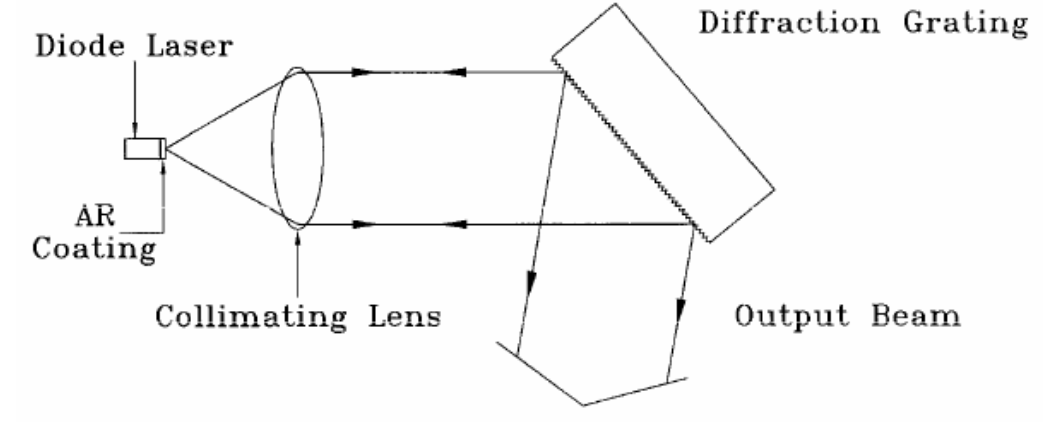
\includegraphics[width=0.8\textwidth]{Littrow Aufbau}
\caption{Littrow Aufbau zur zusätzlich fokussierung des Frequenzbereiches. Der Strahl wird durch eine Sammellinse fokussiert und auf ein Gitter gelenkt, welches so ausgerichtet ist, dass das Maximum erster Ordnung zurück in den Diodenchip reflektiert wird.\cite{teachspin}}
\label{fig:Littrow}
\end{figure}
Da sich im Resonator dadurch eine stehende Welle ausbildet können die Moden die sich dort ausbilden nur Vielfache der doppelten Resonatorlänge $L$ sein.
\begin{equation}
\frac{N\lambda}{2}=L
\end{equation}
\begin{figure}[h]
\centering
\includegraphics[width=0.8\textwidth]{Diodenlaser Verstärkungsfaktoren}
\caption{Einfluss der verschiedenen Faktoren wie internem und externem Resonator auf die Gesamtverstärkung.\cite{teachspin}}
\label{fig:Verstärkung}
\end{figure}
Um die Frequenz des Lasers zusätzlich zu stabilisieren wird ein Littrow-Aufbau wie in Abbildung $\ref{fig:Littrow}$ verwendet. Bei diesem wird eine Sammellinse und ein Beugungsgitter verwendet, welches gemäß der Bragg-Bedingung:
\begin{equation}
\lambda=2d\sin(\Theta)
\end{equation}
mit dem Linienabstand des Gitters $d$, so ausgerichtet wird, dass das Maximum erster Ordnung zurück in den Laser reflektiert wird wodurch ein weiterer externer Resonator entsteht. Die verschiedenen Einflüsse auf die Verstärkung im Resonator ist in Abbildung $\ref{fig:Verstärkung}$ verdeutlicht. Aufgrund der größeren Länge liegen die Maxima des äußeren Resonators deutlich näher beieinander als die des kleineren Resonators.
\begin{figure}[h]
\centering
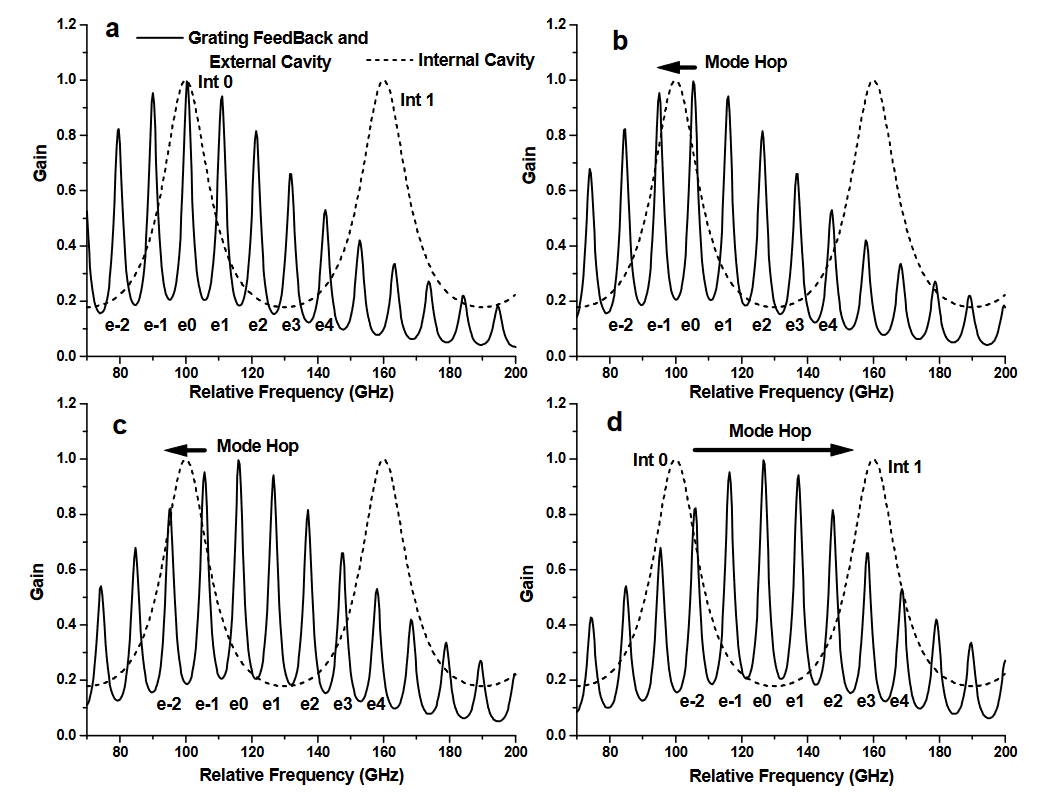
\includegraphics[width=0.6\textwidth]{Mode-hopping}
\caption{Mode-hopping durch Veränderung des Gitterwinkels und somit des externen Resonators.\cite{teachspin}}
\label{fig:Mode-hopping}
\end{figure}
Wegen der komplizierten Überlagerung der unterschiedlichen Verstärkungsfaktoren kann es zum springen des Lasers zwischen verschiedenen Moden kommen. Dieses Phänomen wird Mode-hopping genannt und ist in Abbildung $\ref{fig:Mode-hopping}$ illustriert.
\subsection{Rubidium Spektrum}
\begin{figure}[h]
\centering
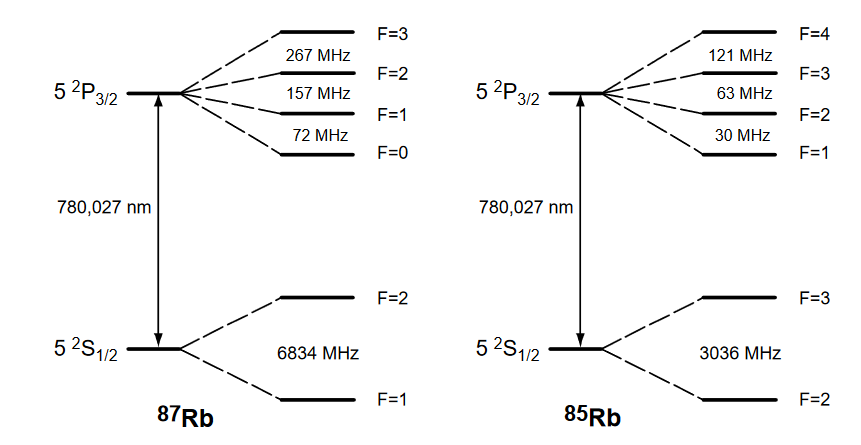
\includegraphics[width=0.45\textwidth]{Rubidium Hyperfeinstruktur}
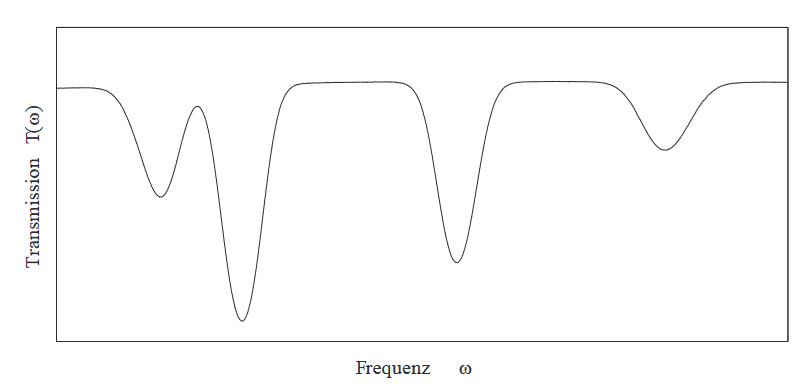
\includegraphics[width=0.45\textwidth]{Rubidium Absorptionsspektrum}
\caption{Energieniveauschema der Hyperfeinstruktur (links) und Absorptionsspektrum (rechts) von Rubidium.\cite{ulm}}
\label{fig:Rubidium}
\end{figure}
Das Absorptionsspektrum von Rubidium sowie die korrespondierende Hyperfeinstruktur sieht aus wie Abbildung $\ref{fig:Rubidium}$ wobei durch dieses Spektrum zwei unterschiedliche Rubidium-Isotope gezeigt werden. Die Wellenlänge der Absorption von Rubidium liegt bei circa $\SI{780}{\nano\meter}$, worauf der Laser eingestellt werden kann. Die Übergänge im Absorptionsspektrum kommen durch die Hyperfeinstruktur zustande, welche durch die Kopplung des Gesamtdrehimpulses des Elektrons $\vec{J}$ und Kerns $\vec{I}$ zum Gesamtdrehimpuls $\vec{F}=\vec{J}+\vec{I}$ zustande kommt. Da die beiden Rubidium Isotope unterschiedliche Kernspins haben zeigen sie auch unterschiedliche Absorptionslinien. Die möglichen Übergänge sind durch die Bedingungen $\Delta F=0,\pm1$ an die Nebenquantenzahl $F$ sowie $\Delta m_F=0, \pm1$ an die magnetische Quantenzahl $m_F$ bestimmt. 